\subsection*{1.1}
%1. Build the circuit shown below using BS170 transistor and a resistor RD = 470 . %Supply
%voltage is VDD = +15 V. Transistor gate is connected to a variable power supply.   
The circuit was built. The resistor, $R_D$, that is defined $470 \omega$  is measured as $462 \omega$.

    %FIG1 CIRCUIT DIAGRAM OF A HALFWAVE RECTIFIER
    \begin{figure}[h!]
        \centering
        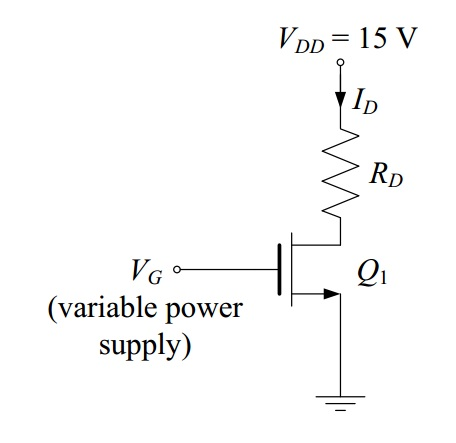
\includegraphics[width=6cm]{circuit_task_1.jpg}
        \captionof{figure}{The circuit in Task 1}
    \end{figure}

\subsection*{1.2}
% 2. Determine the threshold voltage and the transconductance parameter k of the MOS
%transistor. 
%In particular, find the voltage VT for which noticeable drain current appears,
The threshold voltage is determined by observing the drain current whilst increasing the voltage at the gate. When the

%and the voltage VG for which the drain current equals ID0 = 10 mA (use the voltage drop
%across the resistor RD to determine the value of the current). Determine k using the
%formula k = ID0/(VG – VT)2. Note that the parameter k here includes W/L and 0.5 factor
%that you have in the drain current formula ID = 0.5 kn’W/L(VGS–VT)2, i.e., k = 0.5kn’W/L.





